\documentclass[11pt, oneside]{article}   	% use "amsart" instead of "article" for AMSLaTeX format
\usepackage{geometry}                		% See geometry.pdf to learn the layout options. There are lots.
\geometry{letterpaper}                   		% ... or a4paper or a5paper or ... 
%\geometry{landscape}                		% Activate for for rotated page geometry
%\usepackage[parfill]{parskip}    		% Activate to begin paragraphs with an empty line rather than an indent
\usepackage{graphicx}				% Use pdf, png, jpg, or eps� with pdflatex; use eps in DVI mode
								% TeX will automatically convert eps --> pdf in pdflatex		
\usepackage{amssymb}
\usepackage{amsmath}
\usepackage{parskip}
\usepackage{color}

\title{Paraboloid Surface Area}
%\author{The Author}
%\section{}
% \subsection*{R code}
\date{}							% Activate to display a given date or no date

\graphicspath{{/Users/telliott_admin/Dropbox/Tex/png/}}

% \begin{center} 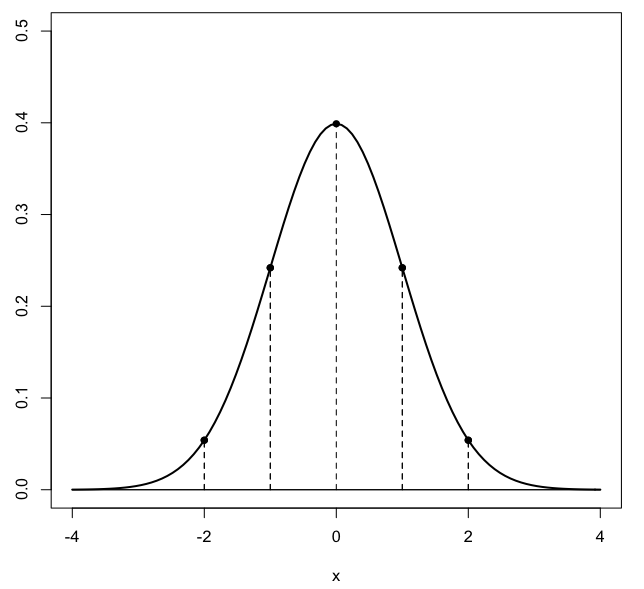
\includegraphics [scale=0.4] {gauss3.png} \end{center}
% \begin{bmatrix} a  &  b \\ c  &  d \end{bmatrix}
% \bigg |_

\begin{document}
\maketitle
\Large

A paraboloid is a solid whose vertical cross-section is a parabola (usually, it is centered along the $z$-axis).  It may be oriented opening up, or down.  The cross-sections parallel to the $xy$-plane are typically circles, though the shape factors for the parabolas in the $xz$- and $yz$-planes could be different, leading to an ellipse for the cross-sections.

Consider
\[ z = 2 - x^2 - y^2 \]

This is a paraboloid that opens down (it gets big when either $x$ or $y$ get large).  The vertex is at $z=2$.  When $z=0$, the cross-section is a circle of radius $r^2=2$.

Usually, cylindrical coordinates are good for dealing with this solid.  For example, the volume element is $dV = \ dz \ r \ dr \ d \theta$.

As with the volume, there are two ways (at least) to do the surface area.  The first is to lay the parabola down as $f(x)$.  

\[ f(x) = \sqrt{x} \]
\[ f'(x) = \frac{1}{2} \frac{1}{\sqrt{x}} \]
\[ f'(x)^2 = \frac{1}{4x} \]

For the surface area of a volume of revolution, we take the circumference of the solid at each value of $x$ times the path element $ds$ (\emph{not} $dx$).  This element is

\[ ds = \sqrt{1 + f'(x)^2} \ dx \]
\[ = \sqrt{1 + \frac{1}{4x}} \ dx \]

So the surface area is

\[ SA = \int_a^b C(x) \ dx \]
\[ = 2 \pi \int _a^b\sqrt{x} \ \sqrt{1 + \frac{1}{4x}} \ dx \]
\[ = 2 \pi \int_a^b \ \sqrt{x + \frac{1}{4}} \ dx \]
\[ = \frac{4}{3} \pi \ (x + \frac{1}{4})^{3/2} \ \bigg |_a^b \]
\[ = \frac{4}{3} \pi \ [  \ (b + \frac{1}{4})^{3/2} -  (a + \frac{1}{4})^{3/2} \  ] \]

If $a=0$ 

\[ = \frac{4}{3} \pi \ [  \ (b + \frac{1}{4})^{3/2} -  \frac{1}{4})^{3/2} \  ] \]
\[ = \frac{4}{3} \pi \ [  \ (b + \frac{1}{4})^{3/2} -  \frac{1}{8} \  ] \]

For this problem, $b=2$ and the answer simplifies a bit

\[ = \frac{4}{3} \pi \ [  \ (2 + \frac{1}{4})^{3/2} -  \frac{1}{8} \  ] \]
\[ = \frac{4}{3} \pi \ [ \frac{27}{8} -  \frac{1}{8} \  ] \]
\[ = \frac{26}{6} \pi \]

Let's try to do this by integrating over two variables.  We have
\[ f(x,y) = 2 - x^2 - y^2 \]
\[ f_x = -2x \]
\[ f_y = -2y \]

The surface area element is

\[ dS = \sqrt{1 + f_x^2 + f_y^2} \ dx \ dy \]

The surface area integral is

\[ SA = \iint_R \sqrt{1 + f_x^2 + f_y^2} \ dx \ dy \]
\[ = \iint_R \sqrt{1 + 4x^2 + 4y^2} \ dx \ dy \]

Now is a good time to switch to polar coordinates (remember the extra factor of $r$):

\[ SA = \int_{\theta = 0}^{2 \pi} \int_{r=0}^{R}  \sqrt{1 + 4r^2} \ r \  dr \ d \theta \]
\[ = 2 \pi  \int_{r=0}^{R}  \sqrt{1 + 4r^2} \ r \  dr  \]
\[ = 2 \pi \  \frac{1}{12} \ [ \ (1 + 4r^2)^{3/2} \ ] \ \bigg |_0^R  \]

Here, recall that $R = \sqrt{2}$, so

\[ = \frac{\pi}{6} ( 27 - 1)  \]
\[ = \frac{26}{6} \pi \]

\end{document}  